\documentclass[a4paper, 10pt, final, garamond]{book}
\usepackage{cours-preambule}

\raggedbottom

\makeatletter
\renewcommand{\@chapapp}{Programme de kh\^olle -- semaine}
\makeatother

\begin{document}
\setcounter{chapter}{24}

\chapter{Du 02 au 05 mai}

\section{Cours et exercices}
\section*{Chimie chapitre 6 -- Réactions d'oxydoréduction}
\begin{enumerate}[label=\Roman*]
    \litem{Oxydants et réducteurs}~: introduction, définition, réactions
        d'oxydoréduction, équilibrage des demi-équations et couples à connaître,
        équilibrage des réactions rédox~; nombre d'oxydation, introduction,
        règles de calcul, interprétation, lien avec la position dans la
        classification périodique.
    \litem{Piles}~: introduction, vocabulaire, potentiel d'électrode, application
        calcul f.é.m., capacité d'une pile.
    \litem{Réactions d'oxydoréduction}~: diagramme de prédominance, sens de
        réaction et diagramme en potentiel standard, calcul des constantes
        d'équilibre, et application, dismutation et médiamutation
\end{enumerate}

\section*{Chimie chapitre 7 -- Diagrammes potentiel-pH}
\begin{enumerate}[label=\Roman*]
    \litem{Influence pH et oxydoréduction}~: potentiel standard apparent,
    convention de tracé, existence d'un précipité.
    \litem{Diagramme $E$-pH de l'eau}~: tracé.
    \litem{Diagramme $E$-pH du fer}~: introduction, attribution, frontières
    horizontales, verticales et droites frontières + bilan.
    \item{Utilisation des diagrammes potentiel-pH}~: stabilité d'une espèce dans
      l'eau, prévision de la faisabilité d'une réaction rédox, cas d'une
      dismutation.
\end{enumerate}

\section{Cours uniquement}
\section*{Thermo. chapitre 1 -- Description d'un système à l'équilibre}
\begin{enumerate}[label=\Roman*]
  \item{Introduction}~: ordres de grandeur, échelles de description.
  \item{Grandeur d'état}~: définition, température, pression, autres exemples,
    variables extensives et intensives, grandeurs massiques et volume molaire.
  \item{Description d'un gaz}~: comportement microscopique, loi du gaz parfait,
    diagramme de \textsc{Clapeyron}.
  \item{Cas des phases condensées}~: définition, équation d'état, ordres de
    grandeur.
\end{enumerate}

\section*{Thermodynamique chapitre 2 -- Premier principe}
\begin{enumerate}[label=\Roman*]
  \item{vocabulaire}~: système, transformations et exemples.
  \item{Énergie interne}~: définition, énergie interne gaz parfait, capacité
    thermique à volume constant, capacité thermique d'une phase condensée.
  \item{Travail des forces de pression}~: expression générale, cas particulier
    isochore et monobare, transformation quasi-statique (définition, exemples de
    diagrammes, corrélation avec l'aire sous la courbe~; application cycle de
    \textsc{Lenoir}), travail électrique.
  \item{Transferts thermiques}~: définition, différents types de transferts
    thermiques, cas particuliers (adiabatique, thermostat), loi de
    \textsc{Laplace}.
  \item{Premier principe de la thermodynamique}~: énoncé.
\end{enumerate}

\section{Questions de cours possibles}
\begin{enumerate}[label=\sqenumi]
    \item Présenter ce qu'est une pile avec l'exemple de la pile
      \ce{Zn^{2+}/Cu}~: schéma, vocabulaire, explication. Déterminer, à l'aide
      de la formule de \textsc{Nerst}, l'anode et la cathode (les potentiels
      standards seront fournis). Établir l'expression de la capacité d'une pile
      en fonction du nombre d'électrons échangés, de l'avancement à l'équilibre
      et du nombre de \textsc{Faraday} à partir de l'exemple de la pile
      \textsc{Daniell}.

    \item Calculer une constante d'équilibre redox en fonction des potentiels
      standards des couples fournis par l'interrogataire~: directement à partir
      de la formule (justifié par un diagramme en $E$\textdegree), \textbf{et}
      en démontrat la formule. Conclure sur la nature de la réaction.

    \item Présenter les phénomènes de dismutation et de médiamutation à partir
      de diagrammes de prédominances d'une part, et de diagrammes en
      $E$\textdegree\ d'autre part. Indiquer comment repérer une dismutation sur
      un diagramme $E$-pH.

    \item Établir et tracer le diagramme potentiel-pH de l'eau. Une attention
      particulière sera portée à l'établissement du lien entre $E$ et pH et à
      l'utilisation des conventions de tracé. On prendra $p_t = \SI{1}{bar}$.

    \item À partir du schéma du diagramme potentiel-pH du fer, attribuer les
      différentes espèces possibles (données) aux domaines. Expliquer comment
      évolue le nombre d'oxydation dans un diagramme $E$-pH. Discuter de la
      stabilité des espèces du fer dans l'eau. Déterminer les pentes des
      droites frontières.

    \item Refaire l'exercice~:
      \begin{figure}[h!]
        \begin{center}
          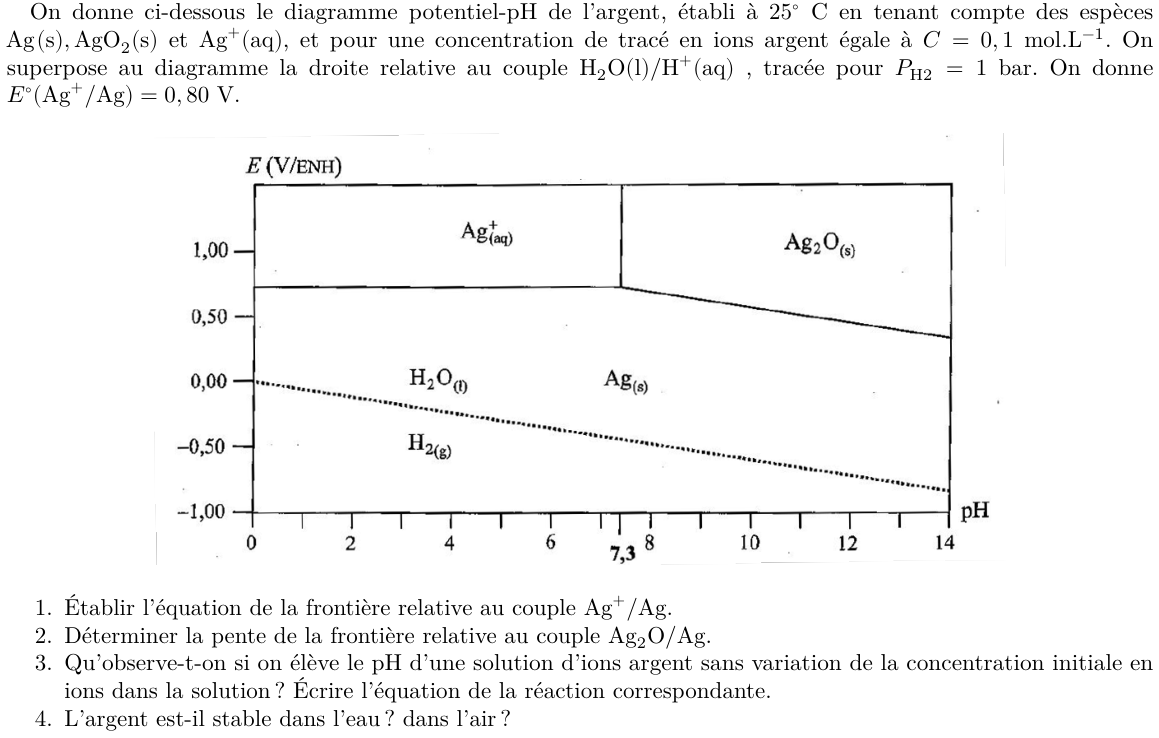
\includegraphics[width=.8\linewidth]{../figures/ch25/ch25_exo1}
        \end{center}
      \end{figure}

    \item Représenter la distribution des vitesses des molécules d'un gaz et ses
      propriétés, définir la vitesse quadratique moyenne et la température
      cinétique.

    \item Présenter le vocabulaire de la thermodynamique~: système isolé, fermé,
      ouvert~; transformations, transformations isochore, monotherme, isotherme,
      monobare, isobare. Définir l'énergie interne d'un système et l'échelle à
      laquelle elle se définit, puis déterminer l'énergie interne d'un gaz
      parfait monoatomique et diatomique, en justifiant les facteurs numériques.

    \item Établir l'expression générale du travail des forces de pression.
    Préciser la nature du système (moteur, récepteur) selon le signe de $W$.
    Présenter le lien avec l'aire sous la courbe d'un diagramme de
    \textsc{Clapeyron}, et mettre en évidence la dépendance de $W$ au chemin
    suivi. Donner la valeur ou l'expression de $W$ pour une transformation
    isochore, pour une transformation monobare, et pour une transformation
    quasi-statique isotherme d'un gaz parfait.

    \item Cycle de \textsc{Lenoir}~: pour une mole de gaz parfait à $P_\Ar =
      \Si{2e5}{Pa}$ et $V_\Ar = \SI{14}{L}$, on effectue les transformations
      suivantes de manière quasi-statique~:
      \begin{enumerate}[label=\alph*)]
        \item chauffage isochore jusqu'à $P_{\rm B} = \SI{4e5}{Pa}$~;
        \item détente isotherme jusqu'à $V_{\rm C} = \SI{28}{L}$~;
        \item refroidissement isobare jusqu'au retour à l'état initial.
      \end{enumerate}
      Calculer $P$, $V$ et $T$ à chaque étape, puis représenter ce cycle sur un
      diagramme de \textsc{Clapeyron}, et calculer les travaux associés aux
      transformations AB, BC et CA et sur le cycle. Conclure sur la nature du
      système.
\end{enumerate}
\vspace{-5pt}

\begin{framed}
    \centering\bfseries\large
    Les fiches doivent être \ul{succinctes} et ne pas faire 3 copies doubles.
    Synthétisez l'information. Il est interdit de copier-coller le cours.
    \bigbreak \Huge
    Les fiches de plus de 2 copies doubles impliqueront un malus de 1 point sur
    la question de cours.
\end{framed}

\end{document}
